\documentclass{beamer}

\usetheme[secheader]{Boadilla}
\usecolortheme{crane}

\usepackage{datetime}

\newdateformat{minimaldate}{%
  \shortmonthname[\THEMONTH] \THEYEAR}

\author[Elahe Dastan]{%
  Elahe Dastan\hfill
  9631025\\
  \texttt{elahe.dstn@gmail.com}
}
\title{Traffic Flow Prediction With Big Data}
\subtitle{A Deep Learning Approach}
\institute[AUT]{Machine Learning\\Amirkabir University of Technology}
\date{\minimaldate\today}

\AtBeginSection[]
{
    \begin{frame}
        \frametitle{Outline}
        \tableofcontents[currentsection]
    \end{frame}
}

\usepackage[style=numeric,sorting=ynt]{biblatex}
\addbibresource{main.bib}

\begin{document}

\begin{frame}
  \titlepage{}
\end{frame}
\begin{frame}
	\frametitle{Outline}
	\tableofcontents{}
\end{frame}

\section{Introduction}

\iffalse
\begin{frame}
	\frametitle{Goal}
	\begin{columns}[t]
		\column{.5\textwidth}
			\begin{definition}
				a service which asks the user to select two points as source and destination on the map and
				service can inform the user \alert{how long it takes} him/her to travel from source to destination.
			\end{definition}
		\pause
		\column{.5\textwidth}
			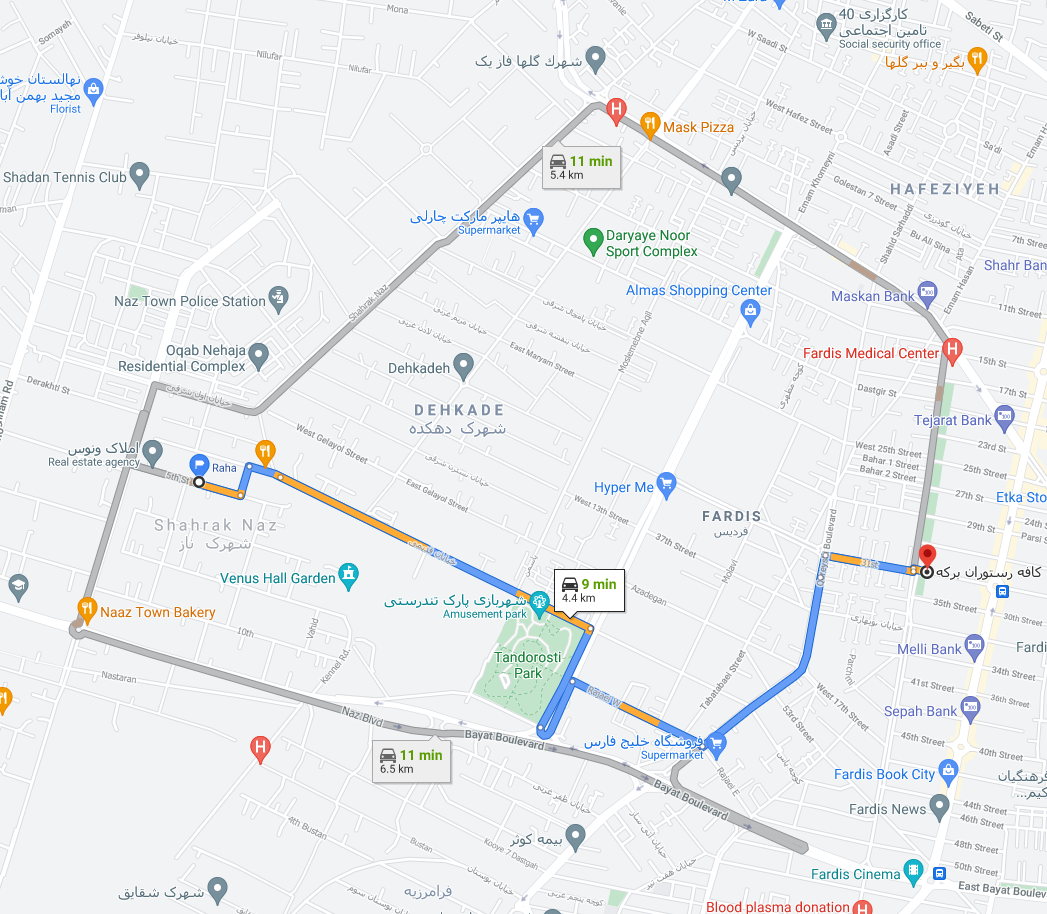
\includegraphics[height=0.5\textheight]{./img/intro.png}
	\end{columns}
\end{frame}
\fi
\begin{frame}
	\frametitle{Goal}
	\begin{columns}
		\column{.5\textwidth}
			\begin{definition}
				predict the speed of traffic in a specific geographical coordinate at a specific time.
			\end{definition}
			\pause
			\begin{example}
				assume you want to go to the university and you want to know the speed of traffic at theater shahr on sunday at 9 am.
			\end{example}
		\pause
		\column{.45\textwidth}
			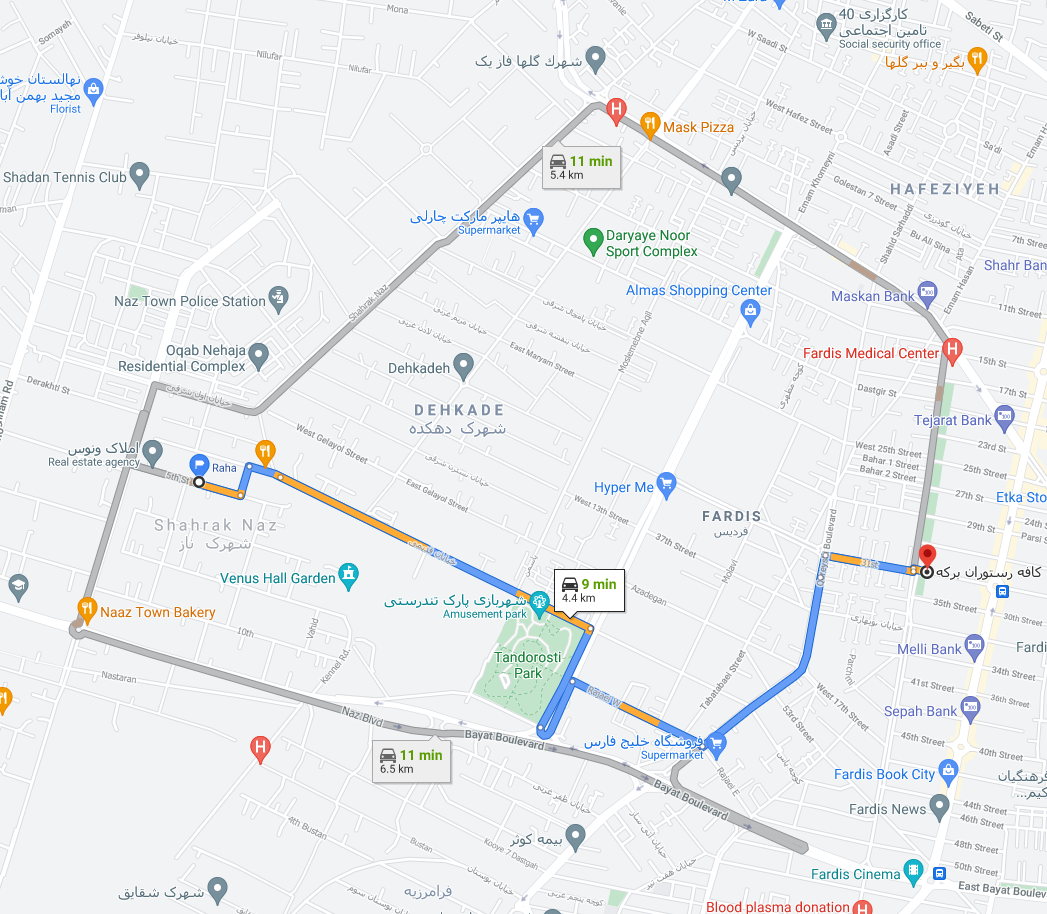
\includegraphics[height=0.5\textheight]{./img/intro.png}
	\end{columns}
\end{frame}
\begin{frame}
  \frametitle{This is done before}
	\begin{columns}
		\column{.25\textwidth}
		
\includegraphics[height=0.5\textheight]{./img/google-maps.png}
		\textbf{Google Maps}\\
		\textit{Google}
		\column{.25\textwidth}
		
\includegraphics[height=0.5\textheight]{./img/waze.png}
		\textbf{Waze}\\
		\textit{Google}
		\column{.25\textwidth}
		
\includegraphics[height=0.5\textheight]{./img/balad.png}
		\textbf{Balad}\\
		\textit{Naghshe Pardazan Ertabatat Novin}
		\column{.25\textwidth}
		
\includegraphics[height=0.5\textheight]{./img/neshan.png}
		\textbf{Neshan}\\
		\textit{Neshan Maps Platform}
	\end{columns}
\end{frame}
\begin{frame}
	\frametitle{Challenges\footnote{\fullcite{2004.08555}}}
  \begin{itemize}
      \item Traffic data is spatio-temporal
      \begin{itemize}
        \item Complex spatial dependencies
        \item Dynamic temporal dependencies
      \end{itemize}
      \item External factors
  \end{itemize}
  \centering
	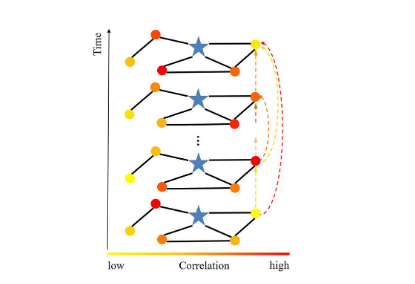
\includegraphics[height=0.5\textheight]{./img/correlations.png}
\end{frame}
\begin{frame}
	\frametitle{How to Calculate Speed?}
  \begin{itemize}
      \item so many people have the app on their cellphones and with the access to their GPSs the traffic flow in a certain street can be estimated periodically
      \item by remembering the traffic flow at the same street at the same day and time in previous weeks the app has a historical model that can be used
  \end{itemize}
\end{frame}
\begin{frame}
  \frametitle{Definition}
  \begin{equation}
    \label{eq:base}
    \hat{v}_{t+1}, \ldots,  \hat{v}_{t+H} = \mathop{\mathrm{argmax}} \log \mathsf{P}({v}_{t+1}, \ldots,  v_{t+H} | v_{t-M+1} , \ldots,  v_{t})
  \end{equation}
  \centering
  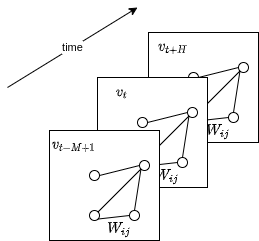
\includegraphics[height=.5\textheight]{img/base.png}
\end{frame}

\section{Solution}

\begin{frame}
	\frametitle{Introduction\footnote{\fullcite{1709.04875}}}
  After years of continuous researches, the research on traffic prediction has achieved great progresses.
  \begin{itemize}
    \item traditional methods: Classical Statistical Methods and Machine Learning Methods
    \item deep learning-based methods: Spatial Dependency Modeling and Temporal Dependency Modeling
  \end{itemize}
\end{frame}
\begin{frame}
	\frametitle{Spatial Dependency}
	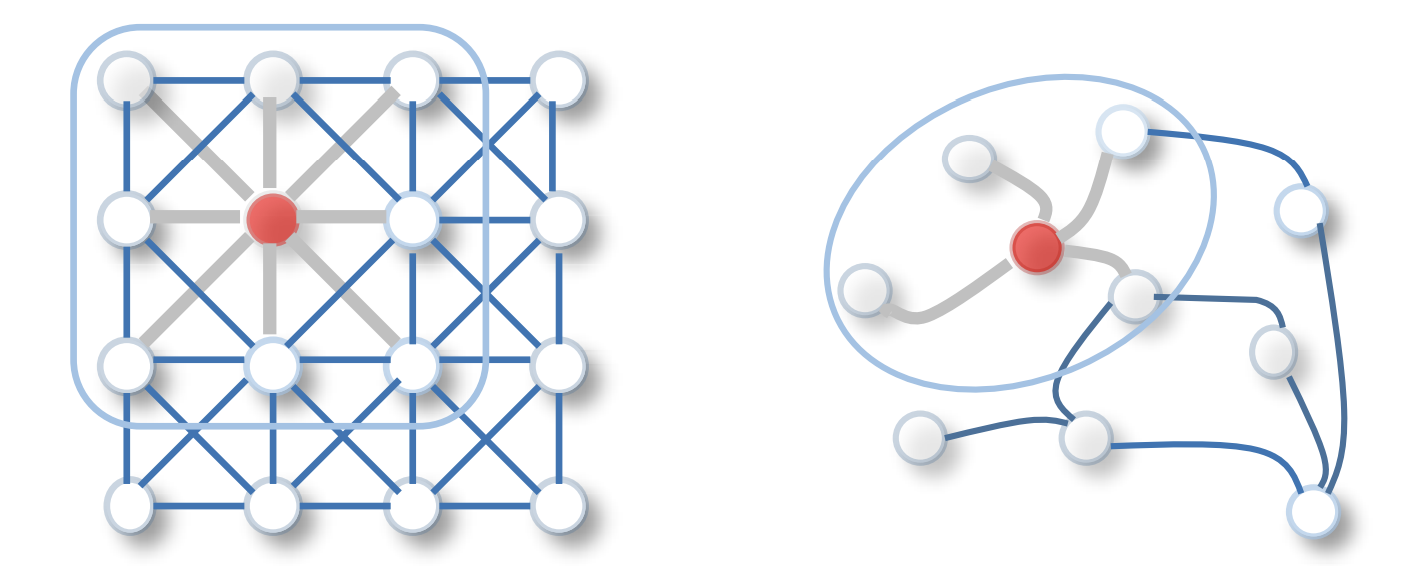
\includegraphics[width=\textwidth]{img/convolution.png}
\end{frame}
\begin{frame}
  \frametitle{Distance}
  \begin{equation}
    W_{i,j} = \left\{
      \begin{array}{ll}
        \exp(-\frac{d^{2}_{ij}}{\sigma^{2}}) & , i \neq j \quad and \quad \exp(-\frac{d^{2}_{ij}}{\sigma^{2}}) \geq \epsilon \\
        0 & , otherwise. \\
      \end{array}\right.
    \label{eq:distance}
  \end{equation}
\end{frame}
\begin{frame}
  \frametitle{Architecture}
  \centering
  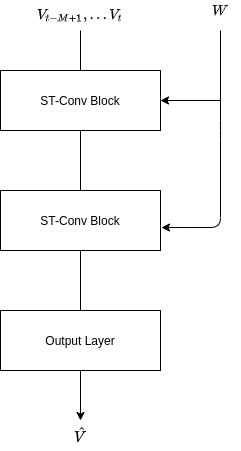
\includegraphics[height=\textheight]{img/blocks.png}
\end{frame}
\begin{frame}
  \frametitle{Architecture}
  \centering
  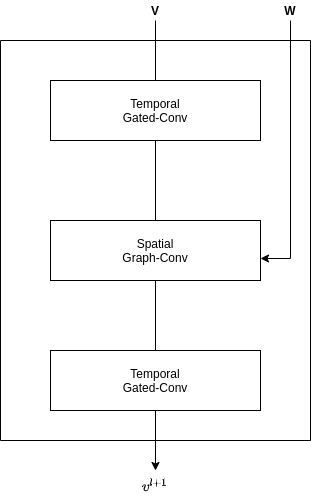
\includegraphics[height=\textheight]{img/inner-blocks.png}
\end{frame}
\begin{frame}[allowframebreaks]
	\frametitle{References}
	\printbibliography
\end{frame}

\end{document}
